\documentclass{article}
\usepackage{tikz}
\usetikzlibrary{arrows.meta,positioning,calc,shapes.geometric}
\pagestyle{empty}
\begin{document}
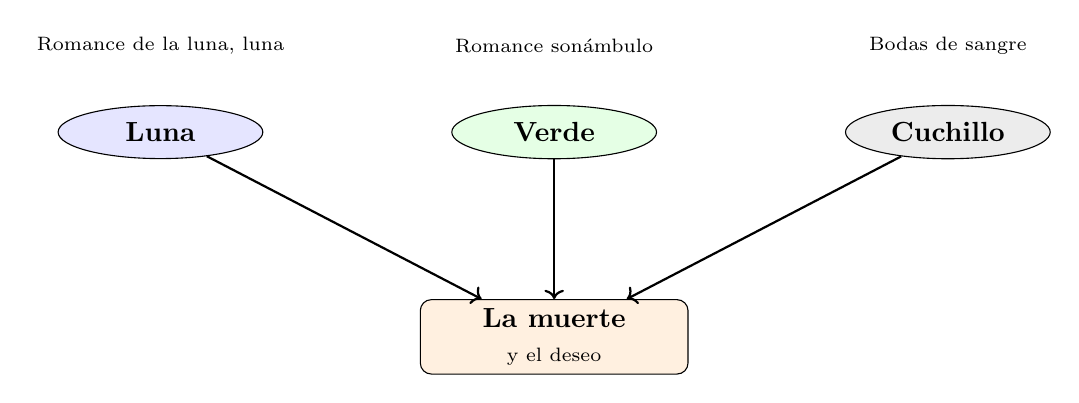
\begin{tikzpicture}
\tikzset{every node/.append style={align=center}}

\node[draw, ellipse, fill=blue!10, minimum width=2.6cm, align=center] (l) at (0,2) {\textbf{Luna}};
\node[draw, ellipse, fill=green!10, minimum width=2.6cm, align=center] (v) at (5,2) {\textbf{Verde}};
\node[draw, ellipse, fill=gray!15, minimum width=2.6cm, align=center] (c) at (10,2) {\textbf{Cuchillo}};
\node[draw, rounded corners, fill=orange!12, minimum width=3.4cm, align=center] (m) at (5,-0.6) {\textbf{La muerte}\\ \scriptsize y el deseo};
\draw[->, thick] (l) -- (m); \draw[->, thick] (v) -- (m); \draw[->, thick] (c) -- (m);
\node[font=\scriptsize, align=center] at (0,3.1) {Romance de la luna, luna};
\node[font=\scriptsize, align=center] at (5,3.1) {Romance sonámbulo};
\node[font=\scriptsize, align=center] at (10,3.1) {Bodas de sangre};

\end{tikzpicture}
\end{document}
